% Options for packages loaded elsewhere
\PassOptionsToPackage{unicode}{hyperref}
\PassOptionsToPackage{hyphens}{url}
\PassOptionsToPackage{dvipsnames,svgnames,x11names}{xcolor}
%
\documentclass[
  ignorenonframetext,
  aspectratio=169]{beamer}
\usepackage{pgfpages}
\setbeamertemplate{caption}[numbered]
\setbeamertemplate{caption label separator}{: }
\setbeamercolor{caption name}{fg=normal text.fg}
\beamertemplatenavigationsymbolsempty
% Prevent slide breaks in the middle of a paragraph
\widowpenalties 1 10000
\raggedbottom
\setbeamertemplate{part page}{
  \centering
  \begin{beamercolorbox}[sep=16pt,center]{part title}
    \usebeamerfont{part title}\insertpart\par
  \end{beamercolorbox}
}
\setbeamertemplate{section page}{
  \centering
  \begin{beamercolorbox}[sep=12pt,center]{part title}
    \usebeamerfont{section title}\insertsection\par
  \end{beamercolorbox}
}
\setbeamertemplate{subsection page}{
  \centering
  \begin{beamercolorbox}[sep=8pt,center]{part title}
    \usebeamerfont{subsection title}\insertsubsection\par
  \end{beamercolorbox}
}
\AtBeginPart{
  \frame{\partpage}
}
\AtBeginSection{
  \ifbibliography
  \else
    \frame{\sectionpage}
  \fi
}
\AtBeginSubsection{
  \frame{\subsectionpage}
}
\usepackage{amsmath,amssymb}
\usepackage{lmodern}
\usepackage{iftex}
\ifPDFTeX
  \usepackage[T1]{fontenc}
  \usepackage[utf8]{inputenc}
  \usepackage{textcomp} % provide euro and other symbols
\else % if luatex or xetex
  \usepackage{unicode-math}
  \defaultfontfeatures{Scale=MatchLowercase}
  \defaultfontfeatures[\rmfamily]{Ligatures=TeX,Scale=1}
\fi
\usetheme[]{Berlin}
\usecolortheme{spruce}
% Use upquote if available, for straight quotes in verbatim environments
\IfFileExists{upquote.sty}{\usepackage{upquote}}{}
\IfFileExists{microtype.sty}{% use microtype if available
  \usepackage[]{microtype}
  \UseMicrotypeSet[protrusion]{basicmath} % disable protrusion for tt fonts
}{}
\makeatletter
\@ifundefined{KOMAClassName}{% if non-KOMA class
  \IfFileExists{parskip.sty}{%
    \usepackage{parskip}
  }{% else
    \setlength{\parindent}{0pt}
    \setlength{\parskip}{6pt plus 2pt minus 1pt}}
}{% if KOMA class
  \KOMAoptions{parskip=half}}
\makeatother
\usepackage{xcolor}
\newif\ifbibliography
\setlength{\emergencystretch}{3em} % prevent overfull lines
\providecommand{\tightlist}{%
  \setlength{\itemsep}{0pt}\setlength{\parskip}{0pt}}
\setcounter{secnumdepth}{-\maxdimen} % remove section numbering
% Input
\usepackage[american]{babel}


% References
\usepackage{natbib}
\usepackage{ebgaramond}
\usepackage[T1]{fontenc}
\usepackage[utf8]{inputenc}
\bibliographystyle{apa}


% Font
\usepackage{palatino} % many other options (eg. tgbonum, times, bookman, lmodern, etc)


% Tables and Figures
\usepackage{float}
\usepackage{caption}
\usepackage{subcaption}
\usepackage{booktabs}
\usepackage{threeparttable}
\usepackage{threeparttablex}
\usepackage{graphicx}
\usepackage{makecell}
\usepackage{multirow}
\usepackage{float}
\usepackage{array}
\usepackage{wrapfig}
\usepackage{tabu}
\usepackage{siunitx} % necessary to compile tables generated by modelsummary in R
\newcolumntype{d}{S[input-symbols = ()]} % necessary to compile tables generated by modelsummary in R
\sisetup{parse-numbers = false}  % Disables parsing of numbers in tables by siunitx.


% Provides easy driver-independent access to several kinds of colors
\usepackage[dvipsnames]{xcolor}


% Other packages
\usepackage{indentfirst} % Indents the first paragraph after a section or subsection
\usepackage{amsmath} % Provides various features to facilitate writing math formulas and to improve the typographical quality of their output
\usepackage[none]{hyphenat} % Disables hyphenation globally


% remove navigation symbols
\setbeamertemplate{navigation symbols}{}


% adjust slides numbers to avoid counting slides in the appendix
\setbeamertemplate{footline}[frame number]{}
\newcommand{\backupbegin}{
   \newcounter{finalframe}
   \setcounter{finalframe}{\value{framenumber}}
}
\newcommand{\backupend}{
   \setcounter{framenumber}{\value{finalframe}}
}


% adjust navigation section name color
\setbeamertemplate{section in head/foot}{\textcolor{yellow}{\hfill\insertsectionhead}}
\setbeamertemplate{section in head/foot shaded}{\textcolor{white}{\hfill\insertsectionhead}}


% adjust bullet points
\setbeamertemplate{itemize items}[default]
\setbeamertemplate{enumerate items}[default]


% Table of Contents with Sections
\setbeamerfont{myTOC}{series=\bfseries, size=\Large}
\AtBeginSection[]{
    \ifnum\value{section}>1
        \frame{
            \frametitle{Roadmap}
            \tableofcontents[current]
        }
    }


% right arrow for subitems
\setbeamerfont{itemize subitem}{size = \small}
\setbeamertemplate{itemize subitem}{$\rightarrow$}

\setbeamertemplate{itemize subsubitem}[square]
\setbeamerfont{itemize subsubitem}{size = \small}



\ifLuaTeX
  \usepackage{selnolig}  % disable illegal ligatures
\fi
\IfFileExists{bookmark.sty}{\usepackage{bookmark}}{\usepackage{hyperref}}
\IfFileExists{xurl.sty}{\usepackage{xurl}}{} % add URL line breaks if available
\urlstyle{same} % disable monospaced font for URLs
\hypersetup{
  pdftitle={Prelimary Results for:},
  pdfauthor={João Pedro Vieira\^{}1},
  colorlinks=true,
  linkcolor={Maroon},
  filecolor={Maroon},
  citecolor={Blue},
  urlcolor={blue},
  pdfcreator={LaTeX via pandoc}}

\title{Prelimary Results for:}
\subtitle{Example for the Reproducible Paper Template: Amazon Priority
Municipalities}
\author{João Pedro Vieira\(^1\)}
\date{May, 2023}
\institute{\(^1\)PUC-Rio}

\begin{document}
\frame{\titlepage}

\begin{frame}{Balanced Event-Study}
\protect\hypertarget{balanced-event-study}{}
\begin{figure}
  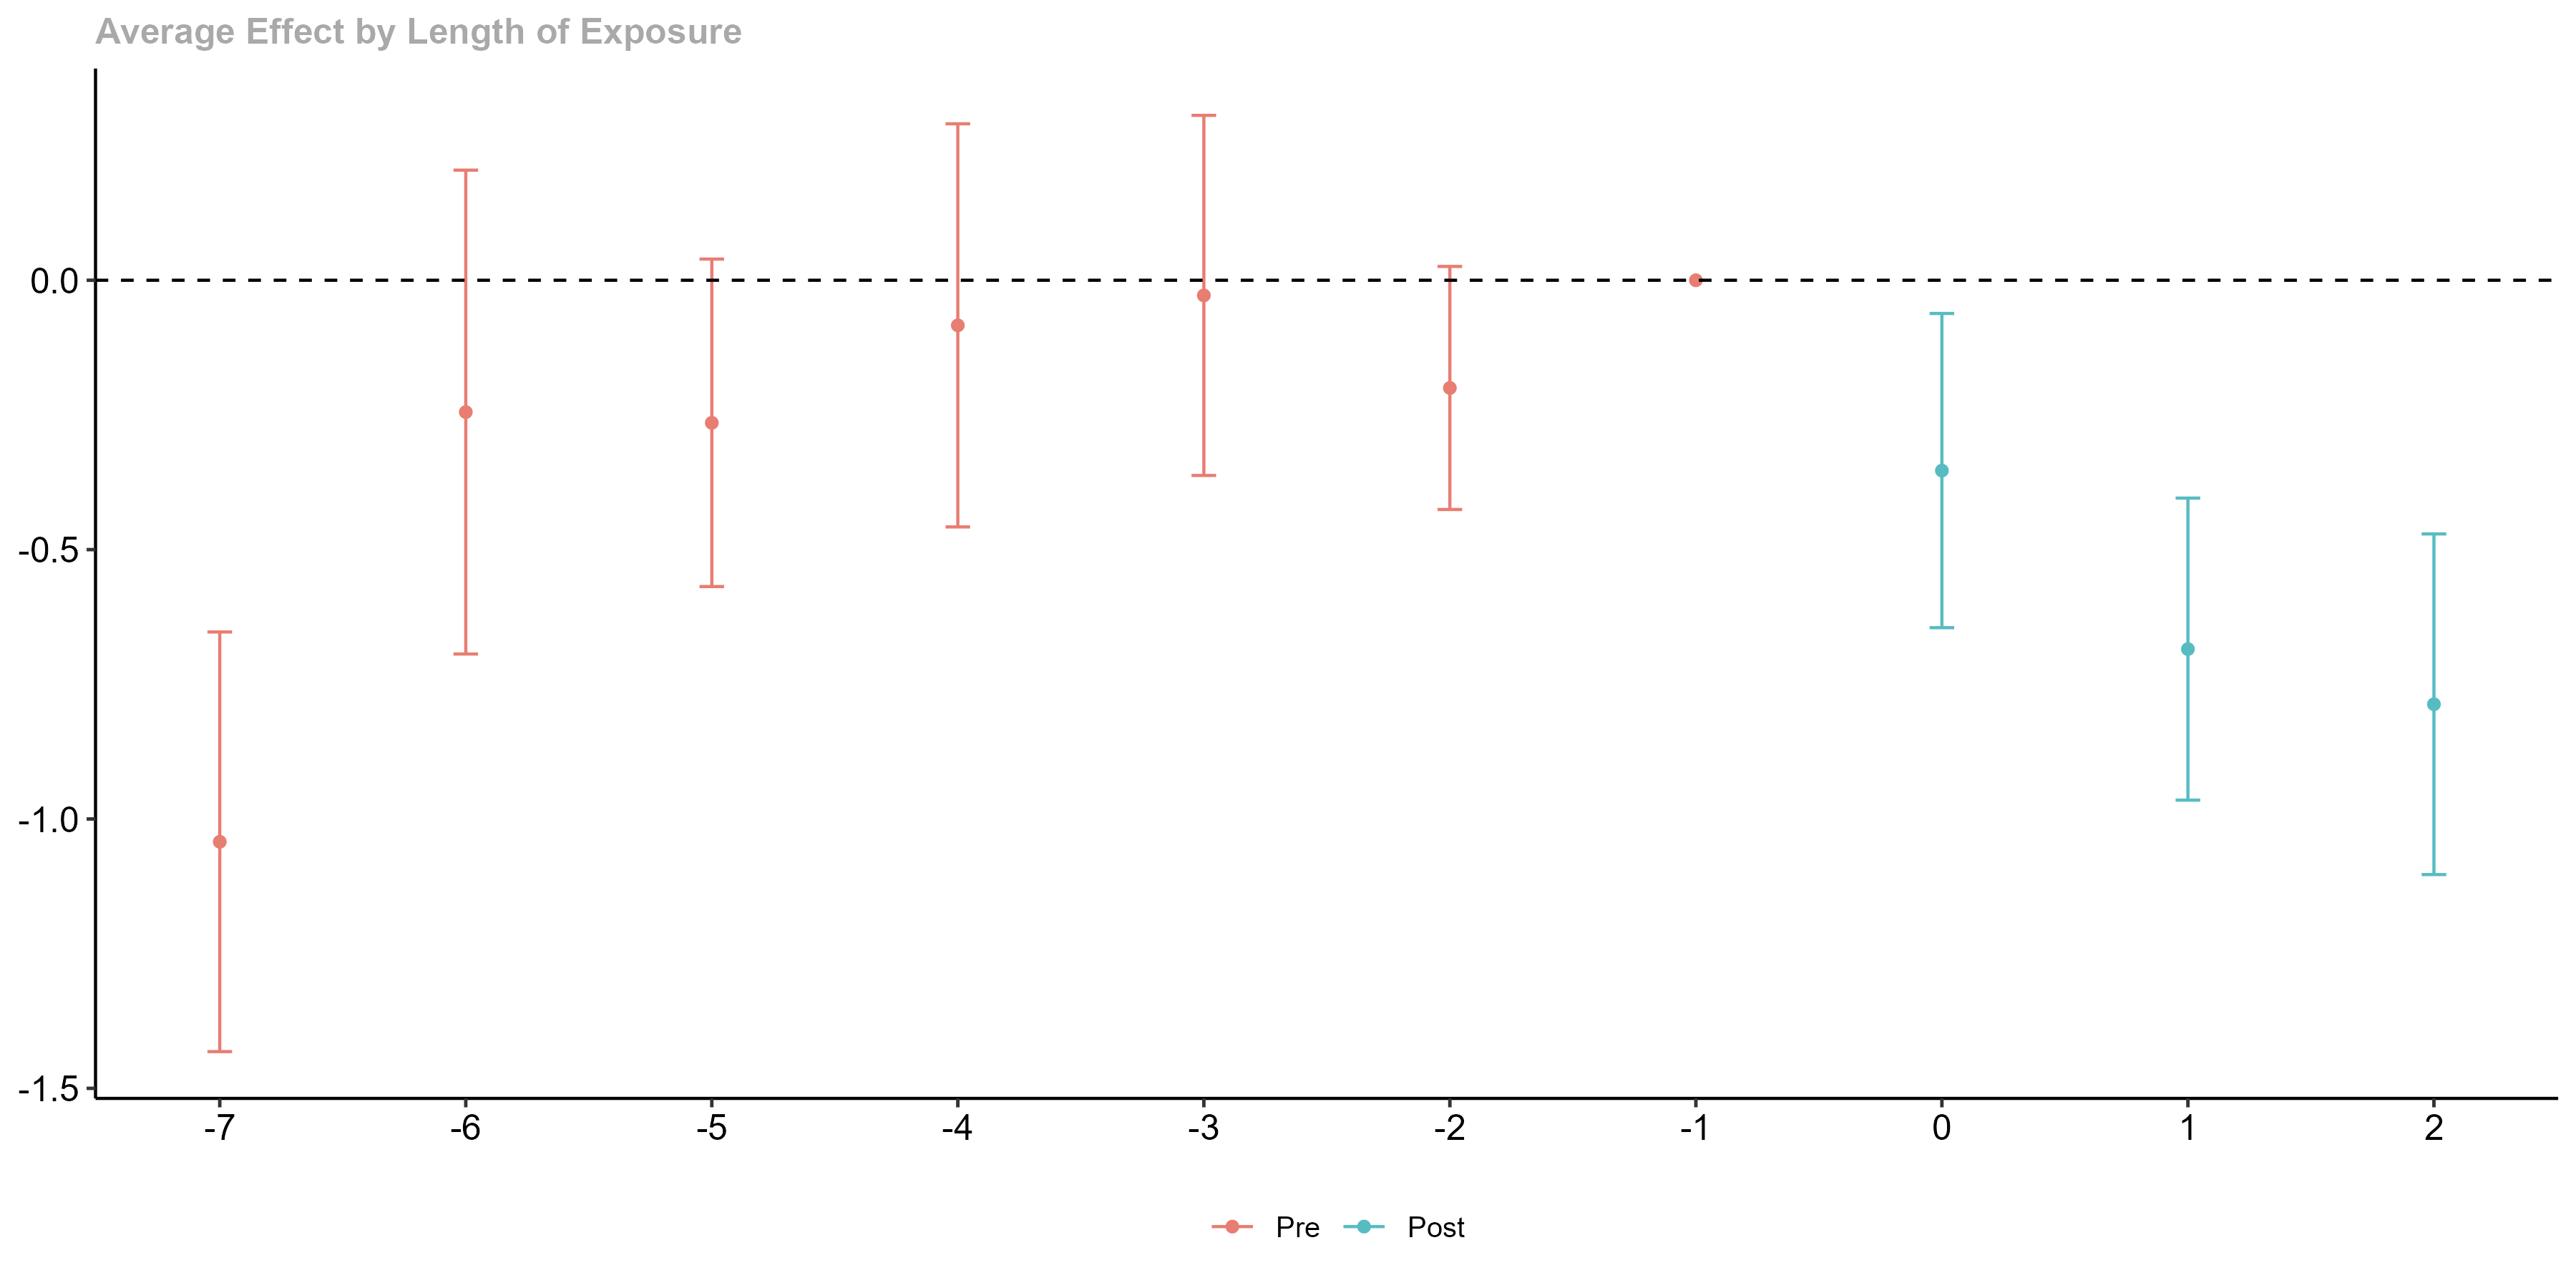
\includegraphics[width=\textwidth]{C:/Users/jpgmv/OneDrive/Projetos/reproducibility_projects/reproducible_paper_example2/results/figures/fig1_eventStudyBalanced.png}
\label{fig:eventStudyBalanced}
\end{figure}
\end{frame}

\begin{frame}{Summary Statistics by Treatment Cohort}
\protect\hypertarget{summary-statistics-by-treatment-cohort}{}
\vspace{-0.5cm}

\begin{table}[H]
\centering
\scalebox{0.6}{
    
\begin{tabular}[t]{l>{\centering\arraybackslash}p{2cm}>{\centering\arraybackslash}p{2cm}>{\centering\arraybackslash}p{2cm}>{\centering\arraybackslash}p{2cm}>{\centering\arraybackslash}p{2cm}c}
\toprule
\multicolumn{1}{c}{} & \multicolumn{5}{c}{Treatment} & \multicolumn{1}{c}{Control} \\
\cmidrule(l{3pt}r{3pt}){2-6} \cmidrule(l{3pt}r{3pt}){7-7}
  & 2008 & 2009 & 2011 & 2012 & 2017 & Never\\
\midrule
Average Annual Deforestation Area in 2000-2007 (1,000 km2) & 0.25 & 0.17 & 0.08 & 0.10 & 0.10 & 0.03\\
 & (0.2) & (0.13) & (0.05) & (0.05) & (0.04) & (0.04)\\
Share of Muni Area in the Amazon (\%) & 95.48 & 94.93 & 80.35 & 100.00 & 100.00 & 89.91\\
 & (9.7) & (14.35) & (36.45) & (0) & (0) & (24.94)\\
Muni Area (1,000 km2) & 21.75 & 11.70 & 7.88 & 13.17 & 30.79 & 6.75\\
 & (29.39) & (5.58) & (7.01) & (1.78) & (24.06) & (13.81)\\
Accumulated Deforestation Area in 2007 (1,000 km2) & 4.45 & 3.89 & 1.84 & 1.24 & 1.82 & 0.95\\
 & (2.48) & (2.57) & (0.95) & (0.85) & (1.1) & (0.91)\\
Forest Area in 2007 (1,000 km2) & 15.40 & 6.15 & 4.55 & 11.08 & 26.07 & 4.15\\
 & (26.78) & (3.63) & (7.02) & (2.89) & (22.7) & (11.04)\\
Non-Forest Area in 2007 (1,000 km2) & 1.34 & 0.53 & 0.90 & 0.05 & 0.91 & 0.80\\
 & (1.62) & (0.73) & (1.73) & (0.06) & (1.41) & (2.12)\\
Hidrography Area in 2007 (1,000 km2) & 0.18 & 0.05 & 0.03 & 0.28 & 0.48 & 0.20\\
 & (0.38) & (0.05) & (0.05) & (0.15) & (0.37) & (0.51)\\
\midrule
Municipalities (\#) & 35 & 8 & 7 & 2 & 8 & 490\\
\bottomrule
\end{tabular}

}
\label{tab:summaryStat}
\end{table}
\end{frame}

\begin{frame}{Unbalanced Event-Study}
\protect\hypertarget{unbalanced-event-study}{}
\begin{figure}
  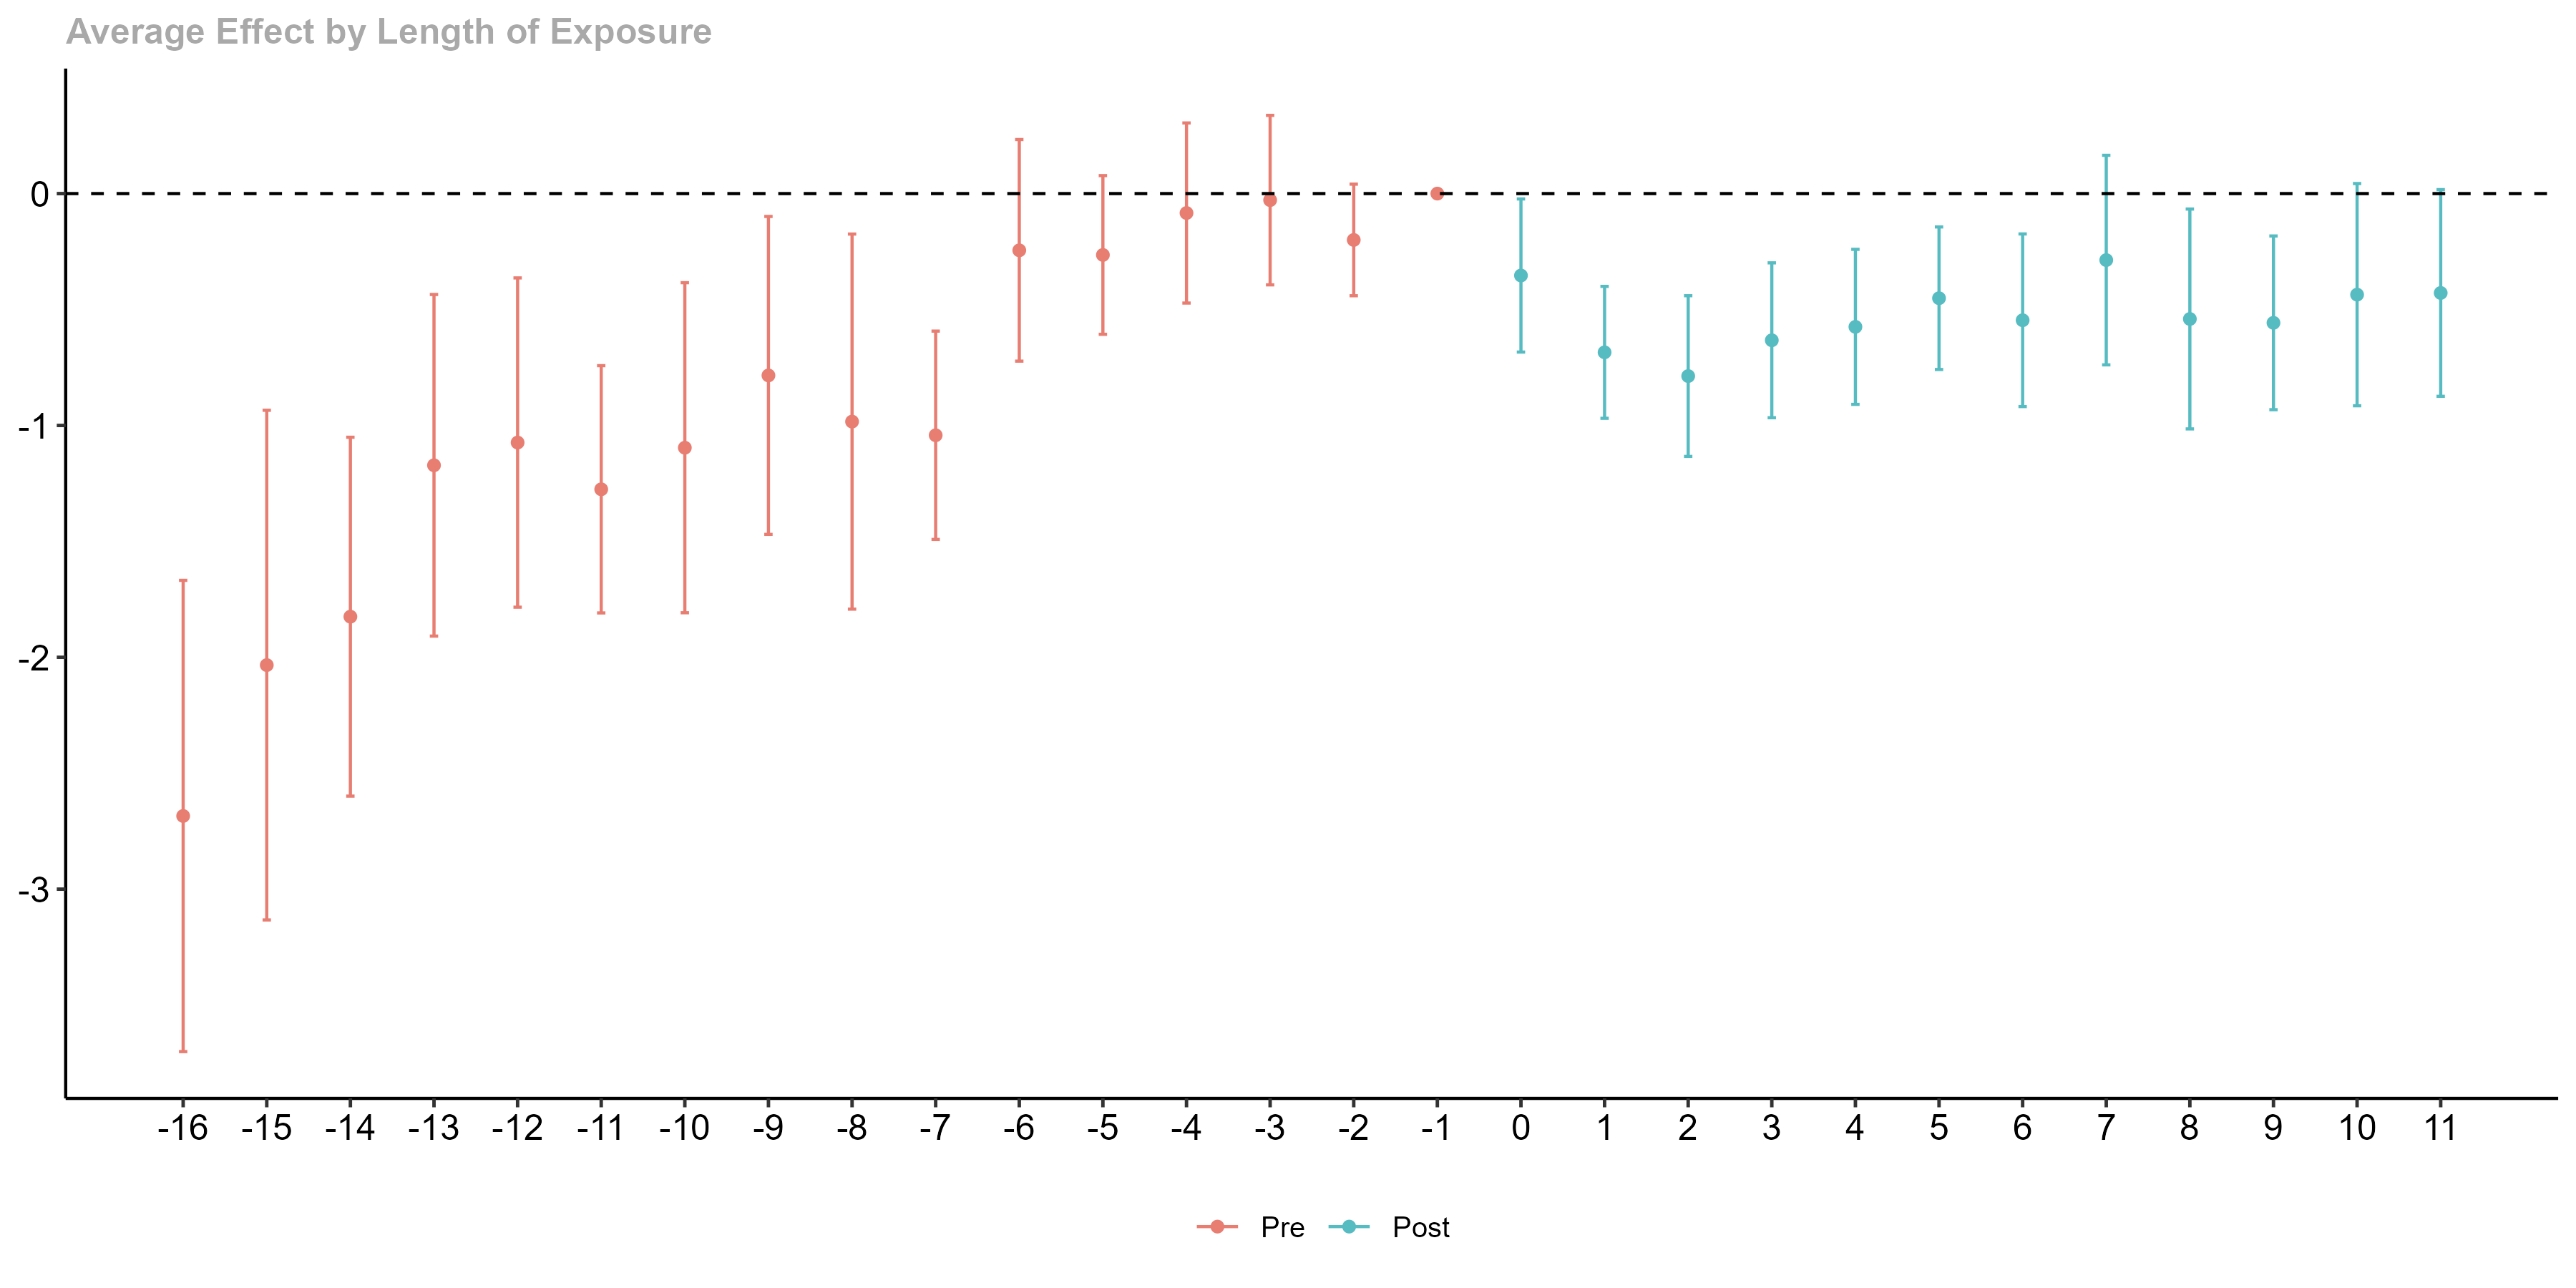
\includegraphics[width=\textwidth]{C:/Users/jpgmv/OneDrive/Projetos/reproducibility_projects/reproducible_paper_example2/results/figures/figA1_eventStudyUnbalanced.png}
\label{fig:eventStudyUnbalanced}
\end{figure}
\end{frame}

\end{document}
